\documentclass[
  paper=a4,
  parskip=half,
  fontsize=12pt,
  listof=toc,
  titlepage,
  headsepline,
  footsepline,
]{scrartcl}

% enable UTF-8 text input
\usepackage[utf8]{inputenc}

% DOCUMENT METADATA

\author{Matthias Traub, Kevin Hoss, Kevin Sieverding, Max ??}
\title{Gartenbewässerungsanlage mit IoT}
\subject{Laborbericht}

% PREAMBLE

%!TeX root = ../index.tex

% BASICS

% make 3rd party packages behave well with scrartcl
\usepackage{scrhack}

% simple arithmetics
\usepackage{calc}

% language support
\usepackage[ngerman]{babel}

% advanced support for quotations
\usepackage[
  autostyle % adapt quote style to document language
]{csquotes}

% color support
\usepackage[dvipsnames,table,hyperref,fixinclude]{xcolor}

% graphics support
\usepackage[]{graphicx}

% extend file name support for graphicx package
\usepackage[
  extendedchars,
  encoding,
  multidot,
  space,
  filenameencoding=utf8,
]{grffile}

% hyperlink support
\usepackage[
  breaklinks,
  pdfusetitle
]{hyperref}

% bibliography support
\usepackage[
  backend=biber,
  style=authoryear,
  labeldate=year,
  sortcites=true,
  sorting=nyt,
  block=space,
  maxnames=2,
  minnames=1
]{biblatex}

% glossaries and acronyms
\usepackage[
    acronym,
    toc=true,
]{glossaries}

% FORMATTING

% micro-typography support (makes most fonts look a little nicer)
\usepackage{microtype}

% support for controlling line spacing
\usepackage{setspace}

% format captions
\usepackage[font=small,labelfont=bf]{caption}

% easily control widow and club penalties
\usepackage[
  defaultlines=4, % keep at least x lines before/after a page break
  all, % apply to whole document
]{nowidow}

% customize list environments
\usepackage{enumitem}

% support for code listings
\usepackage{minted}

% wrapt text around figures
\usepackage{wrapfig}

% MISC

% useful blindtext in document language
\usepackage{blindtext}

% support for placing todo notes in margins
\usepackage[obeyFinal,color=Red,textsize=tiny]{todonotes}


%!TeX root = ../../index.tex

\usepackage[
  %showframe, % draw the layout frame for "debugging"
  top=3cm,
  bottom=2cm,
  left=3.5cm,           % 3.5 + 0.5 Bindingoffset
  right=3cm,
  bindingoffset=0.5cm,
  headheight=22pt,
  headsep=1.25cm-\headheight, % pagetop to header = 1.25cm
  % footheight=\baselineskip,
  footskip=0.75cm, % pagebottom to footer = 1.25cm
  marginparsep=0.3cm,
  marginpar=3.5cm-\marginparsep,
]{geometry}

\setlength{\footheight}{22pt}

%!TeX root=../../index.tex

% include chapter/section titles in headers
\usepackage[
    automark,
]{scrlayer-scrpage}


% Header
\chead[]{}
\ihead[]{}
\ohead[]{\rightmark}

% Footer
\cfoot[]{}
\ifoot[]{}
\ofoot[\pagemark]{\pagemark}

%!TeX root=../../index.tex

%  make \paragraph and \subparagraph behave like small headings
\RedeclareSectionCommands[
    beforeskip=-1sp,
    afterskip=1sp,
    %indent=0pt
]{paragraph,subparagraph}

% Use numbers also for level 1 nested enumerations
\renewcommand{\labelenumii}{\theenumii}
\renewcommand{\theenumii}{\theenumi.\arabic{enumii}.}

%!TeX root = ../index.tex

% support modern fonts
\usepackage[T1]{fontenc}

% sans font that looks similar to Arial
\usepackage{helvet}

% serif font that looks similar to Times New Roman
\usepackage{mathptmx}

% !TeX root = ../../index.tex

\setminted{
  baselinestretch=1.2,
  fontsize=\footnotesize,
  breaklines,
  frame=lines,
  framesep=2mm,
  tabsize=2,
  autogobble
}


% setup hyperref after all packages have been loaded
\hypersetup{
  colorlinks=true,
  allcolors=black,
}

% setup acronyms
% !TeX root = ../index.tex

% \newacronym{cpu}{CPU}{Central Processing Unit}
% \glsunset{cpu}

\newacronym[]{wlan}{WLAN}{Wireless Local Area Network}
\newacronym[]{vm}{VM}{Virtuelle Maschine}
\newacronym[]{iot}{IoT}{Internet of Things}
\newacronym{mom}{MoM}{Message-oriented Middleware}


\makenoidxglossaries{}

% setup bibliography
\addbibresource{assets/bibliography.bib}

% set base path for graphics
\graphicspath{{assets/img}}

% DOCUMENT

\begin{document}

% FRONTMATTER

\maketitle

\clearpage

% use roman page numerals to number frontmatter pages
\pagenumbering{Roman}

% use plain headers
\pagestyle{plain.scrheadings}

% start numbering pages at 2, to include cover page
\setcounter{page}{2}

% use single line spacing to make lists more compact
\singlespacing

\tableofcontents

\clearpage

\listoffigures

\clearpage

% use to change the title of the list of listings
% \renewcommand{\listoflistingscaption}{Quellcodeverzeichnis}
\listoflistings

\clearpage

\setlist[description]{leftmargin=!, labelwidth=4em}

\printnoidxglossary[
    type=\acronymtype,
    sort=nocase,
    nogroupskip,
    nopostdot,
    nonumberlist
]

\setlist[description]{style=standard}

\newcounter{frontpagecount}
\addtocounter{frontpagecount}{\value{page}}

\clearpage

% CONTENT

% use arabic numerals for numbering content pages
\pagenumbering{arabic}

% use the default header style
\pagestyle{scrheadings}

% count content pages from 1
\setcounter{page}{1}

% MS Word does line spacing wrong.
% To get true one-half spacing use '\onehalfspacing'.
% To get something similar to MS Word, use '\setstretch{1.5}'.
\setstretch{1.5}

% !TeX root = ../index.tex

\section{Einleitung}

\subsection{Motivation}
Das \gls{iot} kann in vielen Anwendungsszenarien zum Einsatz kommen, darunter auch in der Gartenbewirtschaftung. Eine effiziente Bewässerung ist von entscheidender Bedeutung, um eine optimale Pflanzenversorgung und Ressourcenschonung zu gewährleisten, insbesondere in Zeiten des Klimawandels und der zunehmenden Wasserknappheit. \gls{iot}-basierte Bewässerungssysteme versprechen eine präzise und bedarfsgerechte Bewässerungssteuerung, die sowohl den Wasserverbrauch reduziert als auch die Pflanzengesundheit und das Pflanzenwachstum fördert.

Gleichzeitig sollen durch den Einsatz von \gls{iot} Routinetätigkeiten automatisiert werden, wodurch für den Nutzer eine erhebliche Zeitersparnis ermöglicht wird.
Dadurch kann der Nutzer gar sorgenfrei in den Urlaub fahren, während das System die Bewässerung übernimmt.

\subsection{Zielsetzung}

In diesem Laborbericht wird ein \gls{iot}-Projekt vorgestellt, das die Konzeption und Implementierung einer intelligenten Gartenbewässerungsanlage zum Ziel hat. Dabei sollen verschiedene Sensoren, Aktoren und Netzwerktechnologien eingesetzt werden, um eine automatisierte, ressourceneffiziente und bedarfsgerechte Bewässerungssteuerung zu ermöglichen. Die Einbeziehung von Umgebungsparametern wie Bodenfeuchtigkeit, Temperatur, Luftfeuchtigkeit und Sonneneinstrahlung soll dabei helfen, den Wasserverbrauch zu optimieren und gleichzeitig die Pflanzenversorgung und -pflege zu verbessern.

\subsection{Aufbau}

Im Rahmen des Laborprojekts werden zunächst in Kapitel \ref{sec:anforderungen} die Anforderungen für ein \gls{iot}-basiertes Bewässerungssystem erarbeitet. Darauf aufbauend soll ein Prototyp in einer simulierten Umgebung entwickelt werden, der die Integration der verschiedenen Komponenten und Technologien demonstriert. Für die Entwicklung des Prototyps wird in Kapitel \ref{sec:architektur} eine passende Systemarchitektur beschrieben. In den darauffolgenden Kapiteln werden die einzelnen Schichten des IoT-Projekts (Hardware-, Netzwerk- und Applikationsschicht) näher beleuchtet.
% !TeX root = ../index.tex

\section{Technische Anforderungen und Systemdesign}

\subsection{Technische Anforderungen}
Nachfolgend werden die technischen Anforderungen an das \gls{iot}-System beschrieben.

\paragraph{Systemübersicht}
Die \gls{iot}-Gartenbewässerungsanlage sollte in der Lage sein, den Wasserverbrauch effizient und automatisch zu steuern, um den Pflanzen im Garten eine optimale Bewässerung zu bieten. Das System sollte aus Sensoren, Aktoren, einer zentralen Steuereinheit und einer Benutzeroberfläche bestehen.

\paragraph{Sensoren}
\begin{itemize}
  \item Boden-Feuchtigkeitssensoren: zur Messung der aktuellen Bodenfeuchtigkeit in verschiedenen Bereichen des Gartens
  \item Boden-Temperatursensoren: zur Messung der aktuellen Bodentemperatur in verschiedenen Bereichen des Gartens
  \item Luft-Feuchtigkeitssensor: zur Erfassung der aktuellen Feuchtigkeit in der Luft
  \item Luft-Temperatursensor: zur Erfassung der aktuellen Umgebungstemperatur in der Luft
  \item Lichtsensor: zur Erfassung der aktuellen Sonneneinstrahlung
\end{itemize}

\paragraph{Aktoren}
\begin{itemize}
  \item Wasserpumpe: zur Beförderung des Wassers aus einer Wasserquelle (z.B. Regenwasserzisterne) in das zu bewässernde Beet
  \item Sonnenschutz: zum Schutz von lichtempfindlichen Pflanzen bei zu starker Sonneneinstrahlung
\end{itemize}

\paragraph{Stromversorgung}
\begin{itemize}
  \item Anschluss an Netzstrom: standardmäßig wird davon ausgegangen, dass das zu bewässernde Gartenbeet Anschluss an den Netzstrom hat
  \item alternative Energiequellen: Solarzellen und/oder Batterien, falls keine Versorgung über Netzstrom möglich ist
\end{itemize}

\paragraph{Kommunikation}
\begin{itemize}
  \item Mikrocontroller: zur Verarbeitung der Sensordaten, Steuerung der Aktoren und Kommunikation über eine Netzwerkschicht
  \item Kommunikationsprotokoll: Wireless Local Area Network (WLAN), um eine drahtlose Verbindung zwischen den Hardwarekomponenten und der Steuereinheit herzustellen
\end{itemize}

\paragraph{Steuereinheit}
\begin{itemize}
  \item Zentraler Server: Steuerung der \gls{iot}-Gartenbewässerungsanlage auf Basis selbst implementierter Funktionslogik
\end{itemize}

\paragraph{Benutzeroberfläche}
\begin{itemize}
  \item Smartphone-App oder Webanwendung: zur Fernsteuerung und Überwachung der \gls{iot}-Gartenbewässerungsanlage, Anzeige von Sensordaten und Einstellung von Bewässerungsparametern
  \item Benachrichtigungsfunktion: um den Benutzer über den aktuellen Systemstatus oder wichtige Ereignisse (z.B. Frostgefahr) zu informieren
\end{itemize}

\paragraph{Softwareanforderungen}
\begin{itemize}
  \item Automatisierung: Die Bewässerungsanlage sollte in der Lage sein, automatisch auf Basis der Sensordaten und vordefinierter Schwellenwerte zu arbeiten
  \item Manueller Modus: Möglichkeit zur manuellen Steuerung der Bewässerung über die Benutzeroberfläche, falls erforderlich
  \item Anpassungsfähigkeit: Die Software sollte in der Lage sein, mit unterschiedlichen Gartenlayouts, Pflanzentypen und Bewässerungszonen umzugehen
\end{itemize}


\subsection{Aufbau der Systemarchitektur}

Für die Umsetzung der technischen Anforderungen wird die in in Abb. \ref{fig:iotschichten} modellierte Systemarchitektur gewählt.

\begin{figure}[h]
  \centering
  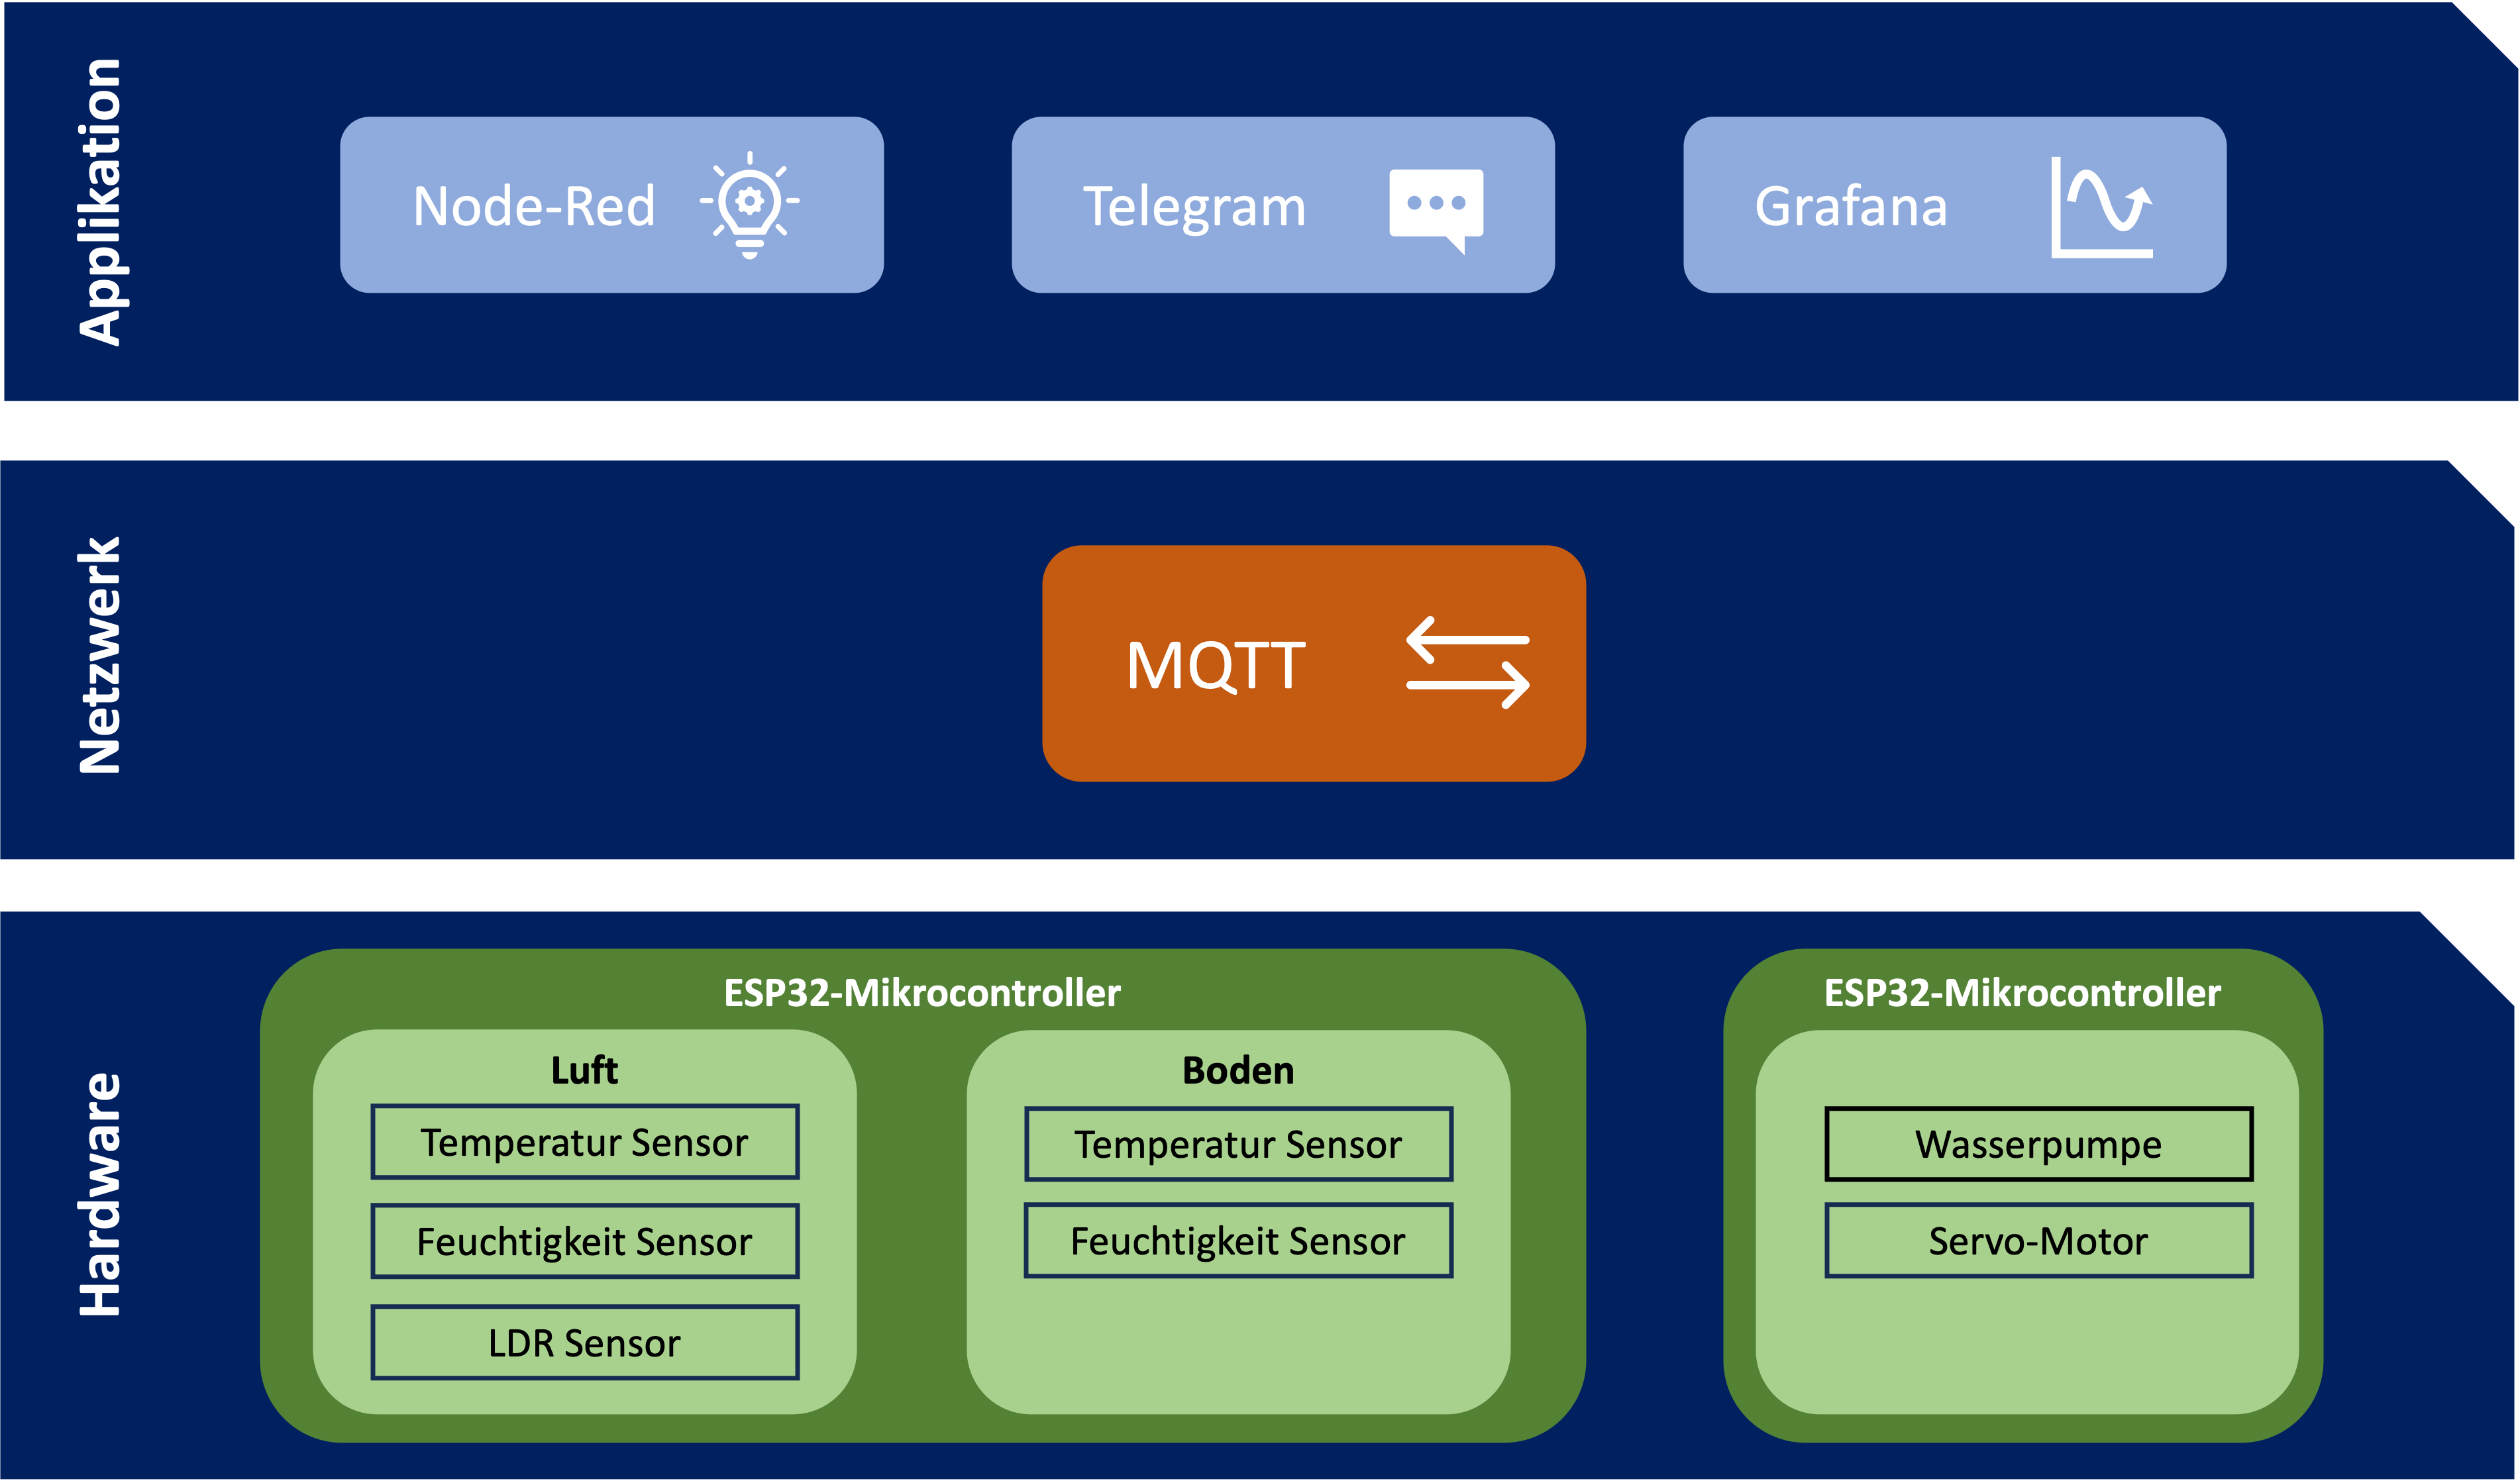
\includegraphics[width=0.8\textwidth]{Aufbau_Architektur.png}
  \caption{Aufbau der IoT-Architektur}\label{fig:iotschichten}
\end{figure}

Auf Hardwareebene kommt ein ESP32-Mikrocontroller zum Einsatz, um die Sensordaten über einen MQTT-Broker zu veröffentlichen. Gleichzeitig wird für die Aktoren ein eigener ESP32-Mikrocontroller eingesetzt, um die Wasserpumpe und Beschattung zu steuern. Die Befehle zur Steuerung der Aktoren werden von dem MQTT-Broker empfangen. Der MQTT-Broker agiert dabei als Vermittler der Nachrichten in der Netzwerkschicht. In der Applikationsschicht wird mit NodeRed die Logik für die \gls{iot}-Steuerung implementiert, über Telegram werden der Benutzer über wichtige Informationen benachrichtigt und in Grafana werden mittels eines Dashboards relevante Daten in Form von Auswertungen für den Nutzer aufbereitet.

Die einzelnen Schichten aus der Systemarchitektur werden in den nachfolgenden Kapiteln näher beschrieben.
% !TeX root = ../index.tex

\section{Bestandteile der Hardwareschicht}

Wie bereits im vorherigen Kapitel angedeutet bildet die Hardwareschicht den untersten Baustein der Systemarchitektur. In diesem Kapitel werden die Methoden vorgestellt, die während des Laborprojekts eingesetzt wurden, um mit der Hardware arbeiten zu können. Desweiteren werden die einzelnen Hardwarebestandteile aufgedrosselt und deren Funktionsweise näher beschrieben.

Beim Arbeiten mit der eingesetzten Hardware haben wir auf die browserbasierte Anwendung Wokwi gesetzt, welche über den Link \textit{https://wokwi.com} erreichbar ist. Die Entscheidung für die virtuelle Umgebung Wokwi wurde aus dem Grund getroffen, da das Aufbauen einer Netzwerkumgebung im Labor nicht möglich ohne Weiteres war. Die Simulation in Wokwi kann allerdings im Anschluss auf die reale Welt übertragen werden und der entwickelte Code läuft auf den entsprechenden Hardwaregeräten ohne eine notwendige Konvertierung.

Bezüglich der eingesetzten Hardware kommen bei unserer intelligenten Gartenbewässerung insgesamt zwei ESP32-Mikrocontroller des Unternehmens Espressif Systems zum Einsatz. Mithilfe der Mikrocontroller können die angeschlossenen Sensoren und Aktoren angesteuert werden. Dabei wird ein ESP32-Mikrocontroller für die Sensoren und einer für die Aktoren eingesetzt. Im folgenden werden vorerst die Sensoren und anschließend die Aktoren näher beleuchtet.

\subsection{Einsatz von Sensoren}
Als Temperatur- und Feuchtigkeitssensor setzen wir in der virtuellen Wokwi Umgebung auf einen DHT22 Sensor. Insgesamt setzen wir davon zwei Stück ein, einen für die Werte in der Luft und einen für die Werte im Boden bzw. in Bodennähe.

In der realen Welt ist der DHT22 Sensor allerdings für die Messung der Bodenfeuchtigkeit nicht geeignet. Grund dafür ist, dass der DHT22 Sensor nicht wasserresistent ist. Im realen Anwendungsfall würde sich ein kapazitiver Bodenfeuchtesensor des Herstellers AZDelivery für die Ermittlung der Feuchtigkeitswerte im Boden anbieten. Die Messsonde wird in den Boden gesteckt und es wird die Feuchtigkeit des Bodens anhand von Veränderungen in der Kapazität gemessen. Ein solcher Sensor verfügt über einen integrierten Verstärker und kann direkt an einen analogen Eingang eines ESP angeschlossen werden. \newline
Für die Messung der Lufttemperatur sollte ebenso bedacht werden, dass der Sensor nicht direktem Niederschlag als auch direkter Sonneneinstrahlung ausgesetzt ist. Entsprechend sollte ein Schutz bzw. eine Umhüllung um den DHT22 Sensor ergänzt werden. Wichtig ist jedoch, dass die Luft weiterhin frei innerhalb des Schutzes zirkulieren kann, um präzise Sensorwerte zu erhalten.\newline
In der Wokwi Umgebung gibt es allerdings nur eine begrenzte Auswahl an Hardwaresensorik. In Wokwi steht der zweite DHT22 Sensor somit für die oberflächennahe Temperatur des Bodens und repräsentativ für die Feuchtigkeit im Boden. Die Werte, die der DHT22 Sensor liefert, werden zum einen in Grad Celsius und zum anderen in Prozent angegeben.

Für die Ermittlung der Helligkeit wird ein LDR-Fotowiderstand Sensor eingesetzt, welcher die Stärke der Sonneneinstrahlung erfasst. Bei dem Umgang bezüglich der Einheit der vom LDR Sensor gelieferten Werte haben sich ein paar Schwierigkeiten aufgetan. Der LDR Sensor liefert auf dem digitalen Output-Pin Werte im Bereich von '0' bis '65535'. Der Wert steigt dabei, wenn die Sonneneinstrahlung schwächer wird, und sinkt, wenn es in der Umgebung heller wird. Der Wert ergibt sich dabei aus dem Widerstand des Sensors und der Spannung, die am Sensor anliegt. Auf die interne Funktionsweise des Sensors wird allerdings im Rahmen dieses Laborberichts nicht weiter eingegangen. Die Herausforderung liegt nun dabei, den gelieferten Wert am digitalen Output-Pin in die Einheit Lux umzurechnen, um damit in der weiteren Entwicklungsarbeit Logiken definieren zu können. In List. \ref{list:LDR_Berechnung} ist ein MicroPython-Ausschnitt dargestellt, der den Wert des LDR Sensors in die Einheit Lux umrechnet.


\begin{listing}[!ht]
\begin{minted}{python3}
ldr_digital_value = ldr.read_u16()
# Convert digital value to lux
ldr_voltage = ldr_digital_value / 65535 * 5
ldr_resistance = 2000 * ldr_voltage / (1 - ldr_voltage / 5)
brightness_value = 
    round(pow(LDR_RL10 * 1e3 * pow(10, LDR_GAMMA) / ldr_resistance, 
        (1 / LDR_GAMMA)))
\end{minted}
\caption{Berechnung des Lux-Wertes aus dem LDR-Fotowiderstand}
\label{list:LDR_Berechnung}
\end{listing}
    

Die drei oben aufgeführten Sensoren werden an einen ESP32-Mikrocontroller angeschlossen, welcher mit dem hausinternen \gls{wlan} verbunden ist. Abb. \ref{fig:wokwi_sensoren} zeigt nochmals zusammenfassend einen visuellen Auszug aus Wokwi, auf dem der Anschluss der Sensorik an den ESP32-Mikrocontroller dargestellt ist. Auf der rechten Seite befinden sich die beiden DHT22 Sensoren, auf der linken Seite der LDR-Fotowiderstand Sensor und in der Mitte der ESP32-Mikrocontroller.

\begin{figure}[h]
    \centering
    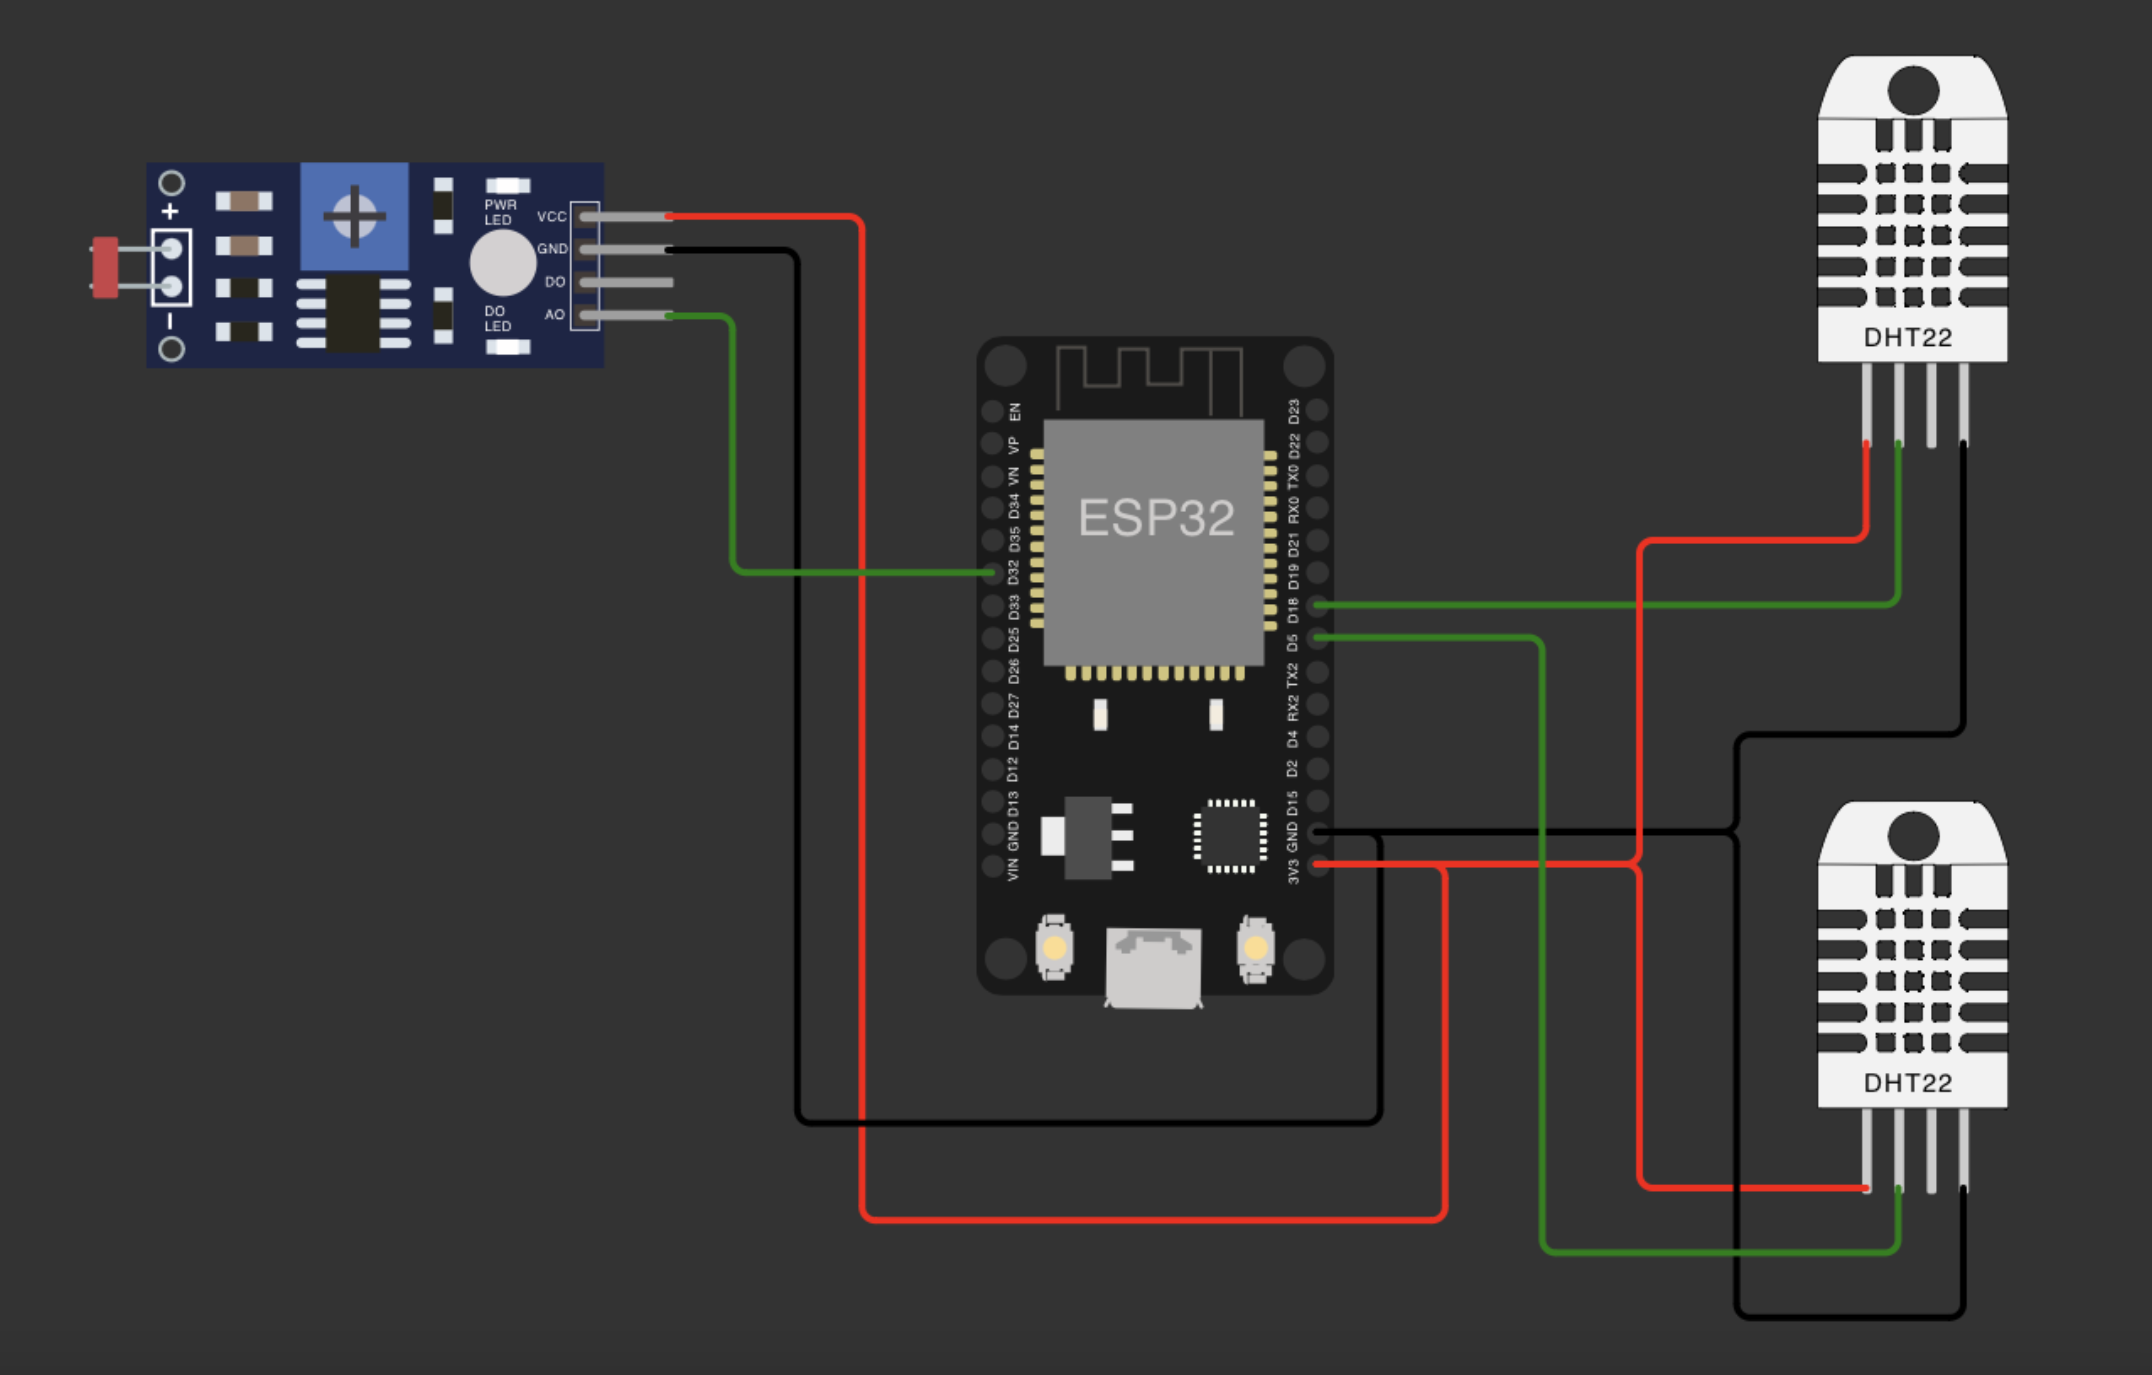
\includegraphics[width=0.8\textwidth]{Wokwi_Sensoren.png}
    \caption{Anschluss der Sensorhardware in der virtuellen Umgebung Wokwi}\label{fig:wokwi_sensoren}
\end{figure}

\subsection{Einsatz von Aktoren}
Bezüglich der Steuerung der Markise, um die Sonneneinstrahlung zu reduzieren, verwenden wir einen Servo-Motor, der die Markise aus- und einfahren kann. Die Steuerung des Servo-Motors läuft über die MicroPython Library \textit{Servo}. Über die Angabe eines Winkels bewegt sich der Servo-Motor in die gewünschte Position. Somit kann die Markise über die Drehung des Motors um einen bestimmten Winkel ein- bzw. ausgefahren werden.

Die Steuerung der Wasserpumpe übernimmt ein Relais, welches durch das Schalten eines neuen Stromkreises die Wasserpumpe an- bzw. ausschalten kann. In MicroPython definieren die Werte '0' und '1' des Relais, ob der Stromkreis geschlossen oder offen ist. In Wokwi haben wir zu Demonstrationszwecken eine LED an das Relais angeschlossen, um zu veranschaulichen, ob die Wasserpumpe läuft oder nicht. Im realen Anwendungsfall wird an das Relais anstatt der Wokwi-LED eine Wasserpumpe angeschlossen.

Die beiden Aktoren Servo-Motor und Relais sind an einen ESP32-Mikrocontroller angeschlossen, welcher zusammen mit dem Mikrocontroller der Sensoren mit dem hausinternen \gls{wlan} verbunden ist. Abb. \ref{fig:wokwi_aktoren} zeigt nochmals, analog zum vorherigen Unterkapitel, einen Ausschnitt aus Wokwi, auf dem die Verkabelung der Aktoren mit dem ESP32-Mikrocontroller dargestellt ist. Am oberen Bildrand befindet sich der Servo-Motor, am unteren Bildrand das Relais mit angeschlossener LED und links der ESP32-Mikrocontroller. Im Anhang in List. \ref{list:wokwi_aktoren1}ff. findet sich der Quellcode zu der Python-Implementierung für diesen ESP.

\begin{figure}[h]
    \centering
    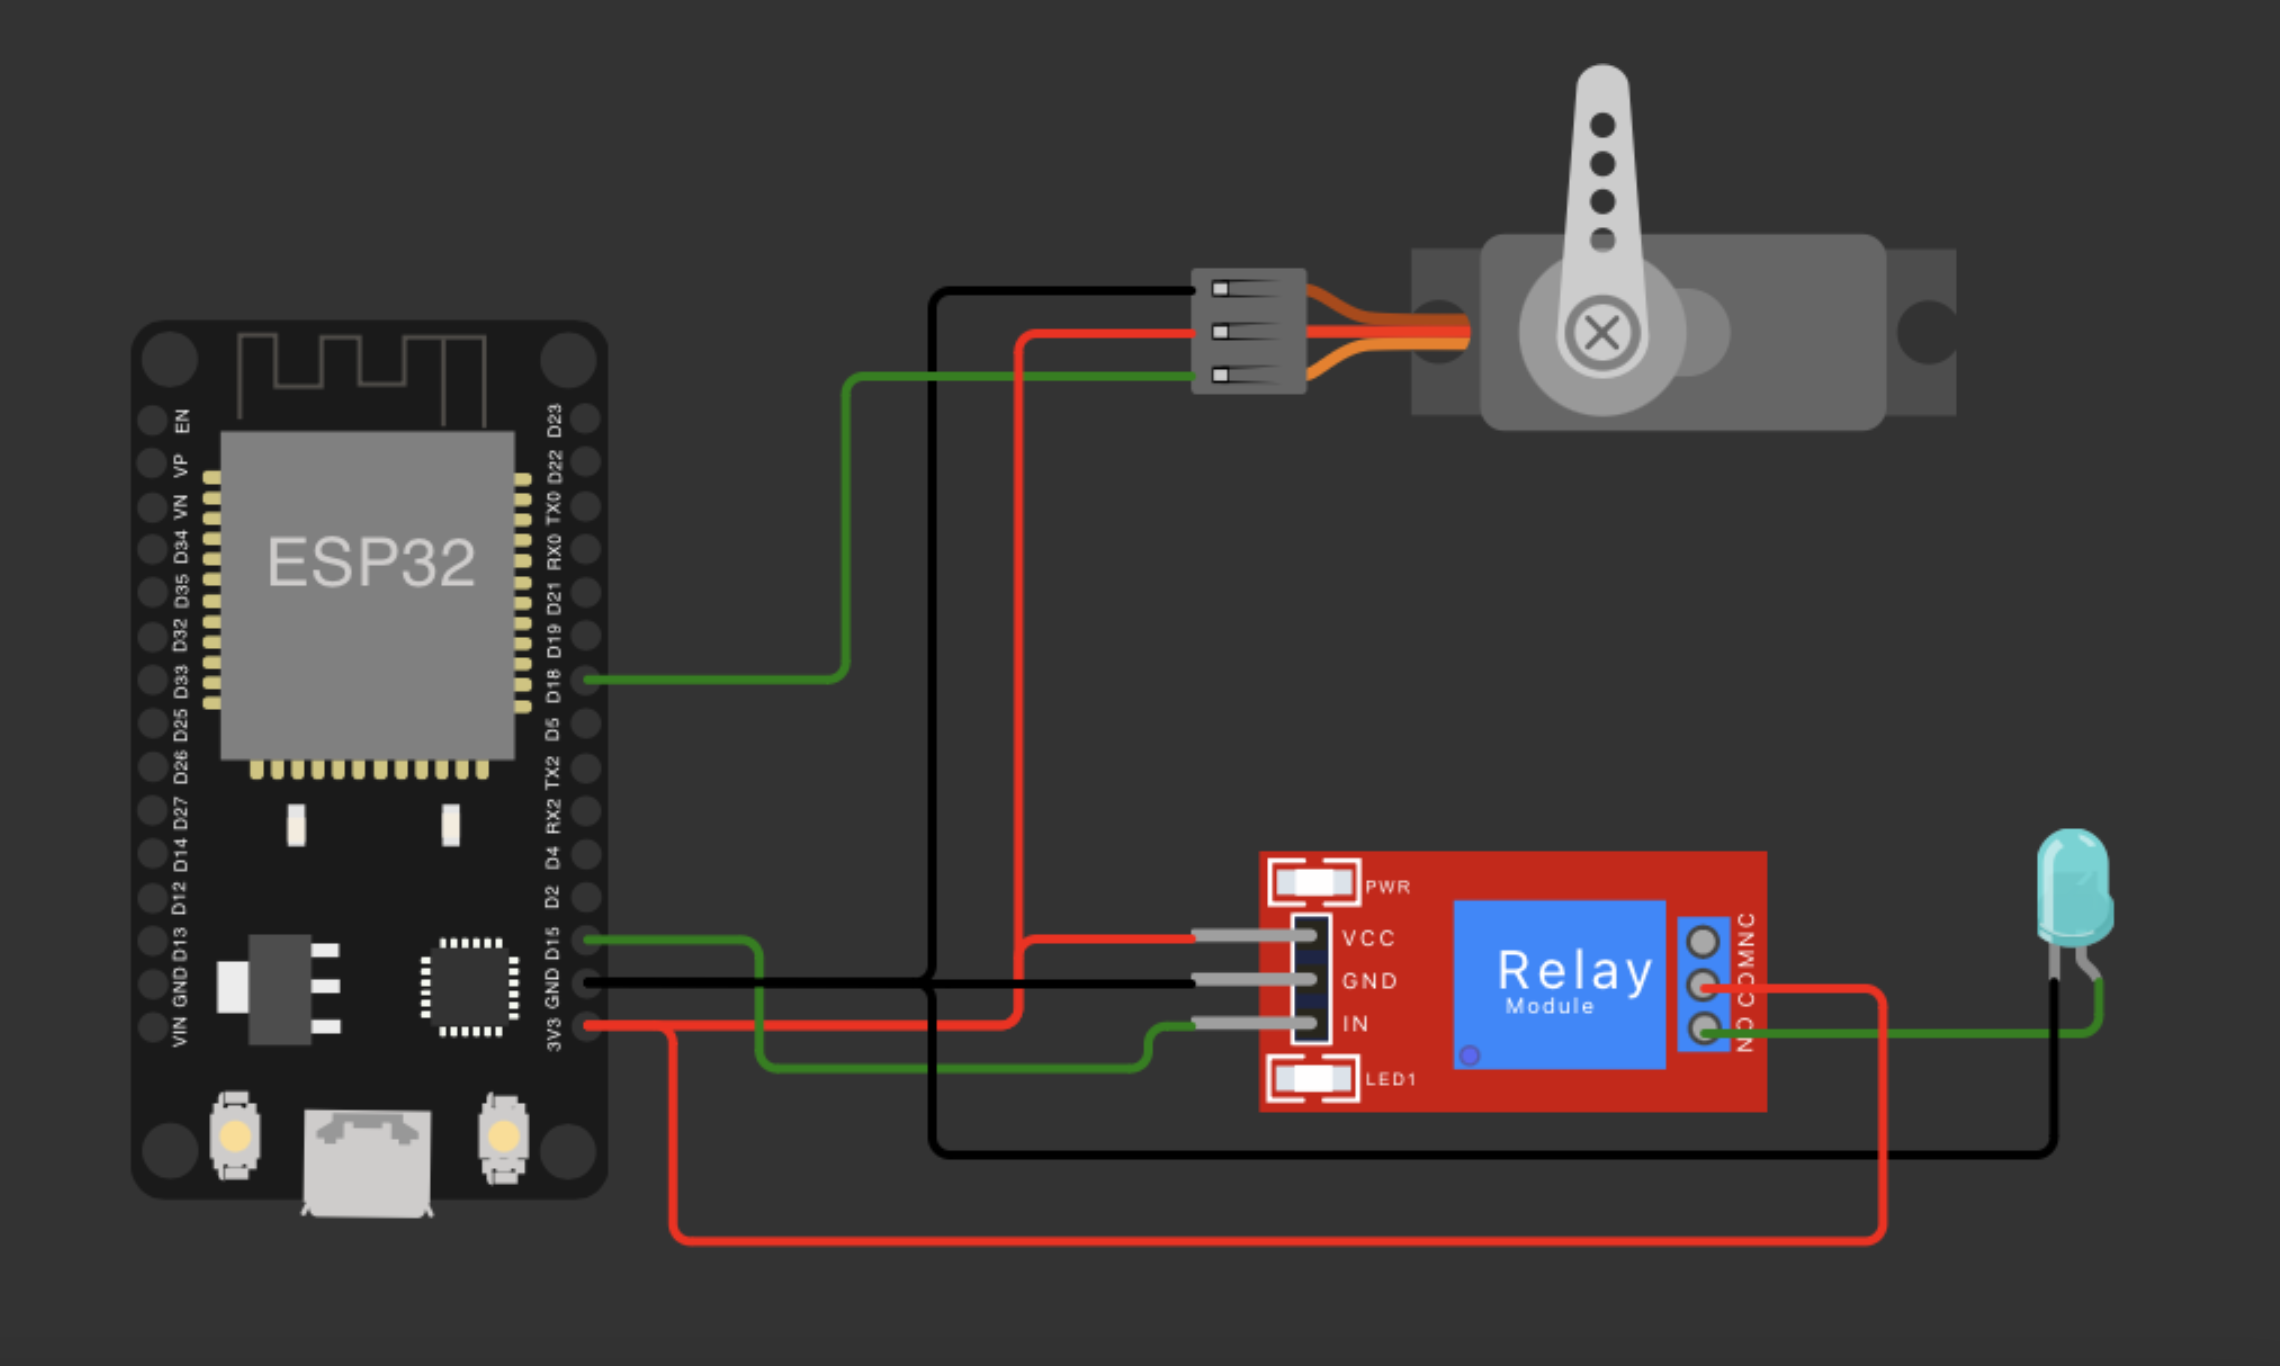
\includegraphics[width=0.8\textwidth]{Wokwi_Aktoren.png}
    \caption{Anschluss der Aktorenhardware in der virtuellen Umgebung Wokwi}\label{fig:wokwi_aktoren}
\end{figure}
% !TeX root = ../index.tex

\section{Netzwerkschicht}

Die Aufgabe der Netzwerkschicht ist es die verschiedenen Mikrocontroller mit der Applikationsebene zu verbinden.
Hierzu sind die Mikrocontroller hierzu, wie bereits beschrieben, mit einem WLAN verbunden, welches ihnen Zugriff auf das öffentliche Internet gewährt.

Dort können sie sich mit einem MQTT-Broker verbinden, welcher als \gls{mom} Teil der Netzwerkschicht bildet und den einfachen Austausch von Daten zwischen den Controllern und der Anwendungsschicht ermöglicht.
Eine funktionale und übersichtliche Gestaltung der Topics ist dabei wichtig für die Verständlichkeit des Systems, weswegen die Topics des Systems einer klaren Struktur folgen:

\begin{minted}{text}
  plantzz/client
  plantzz/temperature/ground
  plantzz/temperature/air
  plantzz/humidity/ground
  plantzz/humidity/air
  plantzz/brightness
  plantzz/pump/state
  plantzz/pump/command
  plantzz/canvas/state
  plantzz/canvas/command
\end{minted}

Die Sensor-Controller schreiben ihre Messwerte zu den dazugehörigen Topics, wie zum Beispiel \texttt{plantzz/temperature/ground}, während die Aktor-Controller auf den Command-Topics hören, um Kommandos zu empfangen und ihren aktuellen status auf die State-Topics schreiben.
Zudem schreiben alle Controller ihren aktuellen Status auf das \texttt{plantzz/client} Topic und registrieren einen Last Will, damit der Status auch im Falle eines Verbindungsverlustes zum Controller aktualisiert wird.

% !TeX root = ../index.tex

\section{Bestandteile der Applikationsschicht}

Die Aufgaben der Anwendungsschicht sind es, die von den Sensoren gesammelten Daten zu speichern und auf diesen aufbauend die Aktoren zu steuern.
Zu diesem Zweck wird die Low-Code/No-Code Plattform Node-RED eingesetzt. Die Plattform erlaubt es über eine einfache, grafische Benutzeroberfläche Programmabläufe zu gestalten und bietet viele vorgefertigte Integrationen zu Softwarelösungen, welche im \gls{iot} beliebt sind.
Beispiele zu vorgefertigten Integrationen sind MQTT und die Time-Series-Datenbank InfluxDB.
Letztere wird ebenfalls im Rahmen dieser intelligenten Gartenbewässerung zur Speicherung und Auswertung der Sensorwerte eingesetzt. Eine \gls{vm} in der Computing-Infrastruktur der DHBW Mannheim dient dazu, um eine Instanz der Plattform Node-RED und eine InfluxDB darauf zu installieren. Für die Visualisierung der wichtigsten Informationen in der Gartenbewässerungsanlage wird eine Grafana-Service ergänzt. 
In einer Container-Umgebung mit \textit{Docker} lassen sich die entsprechende Services einfach starten. \textit{Docker Compose} eignet sich hierbei zum Definieren und Ausführen von mehreren verschiedenen Docker-Anwendungen. Die Compose-Datei aus diesem Laborprojekt ist in List. \ref{list:docker} dargestellt. Das Setup 

\begin{listing}[!ht]
\begin{minted}{python3}
node-red:
influxdb-config:
influxdb-data:
grafana_storage:

services:
node-red:
  image: nodered/node-red
  container_name: node-red
  restart: unless-stopped
  volumes:
    - node-red:/data
  ports:
    - 80:1880
influxdb:
  image: influxdb
  container_name: influxdb
  restart: unless-stopped
  volumes:
    - influxdb-config:/etc/influxdb2
    - influxdb-data:/var/lib/influxdb2
  ports:
    - 8086:8086
  env_file: .env-influxdb
grafana:
  image: grafana/grafana-enterprise
  container_name: grafana
  restart: unless-stopped
  volumes:
    - grafana_storage:/var/lib/grafana
  ports:
    - 3000:3000
\end{minted}
\caption{Definition der Container in docker-compose.yml}
\label{list:docker}
\end{listing}  

In der Node-RED-Umgebung sind die folgenden Anwendungsszenarien umgesetzt: Speicherung der Sensordaten, Steuerung der Pumpe, Steuerung der Markise und die Interaktion mit dem Nutzer über einen Bot des Messenger-Dienstes Telegram.

Die Logik zur Speicherung der Sensordaten ist simpel. 
Je ein Programmablauf in Node-RED hört auf die Topics der verschiedenen Sensorwerte, bringt die Daten in ein passendes Format und schreibt sie in die InfluxDB.
Die Steuerung von Wasserpumpe und Markise sind allerdings komplexer und werden daher im Folgenden nochmal im Detail beschrieben.

\subsection{Steuerung der Wasserpumpe}

Das System soll selbstständig in regelmäßigen Abständen überprüfen, ob die Bodenfeuchtigkeit unter 25\% liegt.
Ist dies der Fall und ist für die nächsten 24 Stunden kein Niederschlag vorhergesagt, so soll die Pumpe aktiviert werden.

Die Pumpe soll für zwei Minuten laufen, um den Boden zu bewässern, und anschließend wieder deaktiviert werden. Damit das Wasser Zeit zum Versickern hat, soll die Prüfschleife für fünf Minuten nach Aktivieren der Pumpe ausgesetzt werden.

\begin{figure}[h]
  \centering
  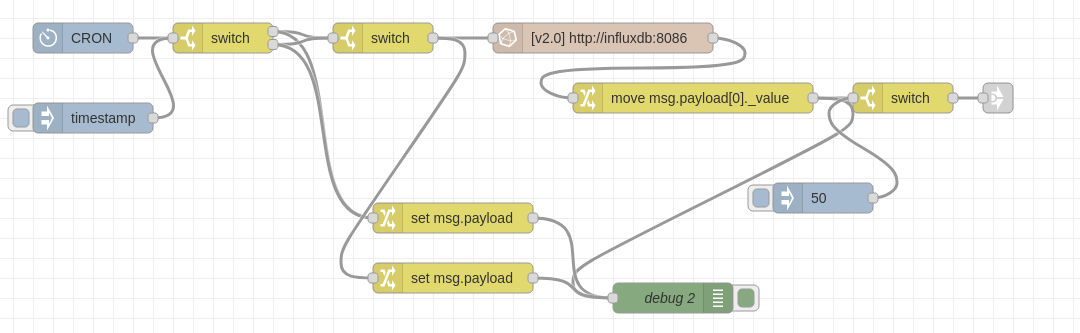
\includegraphics[width=\textwidth]{pump-activation.png}
  \caption{Überprüfungslogik für die Wasserpumpe in Node-RED}\label{fig:pump-activation}
\end{figure}

Abb. \ref{fig:pump-activation} zeigt einen Screenshot der Überprüfungslogik für die Pumpe in Node-RED.
Der Workflow wird jede Minute von dem CRON-Trigger gestartet und überprüft zunächst, ob ein globales Flag gesetzt ist, welches die Überprüfung aussetzten würde.
Darauffolgend wird kontrolliert, ob für die nächsten 24 Stunden Niederschlag vorhergesagt ist.
Die Wetterdaten hierzu werden in einem separaten Workflow mittels eins CRON-Jobs jede Stunde von der öffentlichen Programmierschnittstelle des Deutschen Wetterdienstes geladen und in einer globalen Variable gespeichert.

Falls kein Niederschlag vorhergesagt ist, wird der durchschnittliche Bodenfeuchtigkeitswert der letzten fünf Minuten aus der InfluxDB ermittelt.
Liegt dieser Wert unter 25\%, wird die Steuerungslogik für die Pumpe in einem Sub-Workflow ausgeführt.
Dieser Sub-Workflow ist in Abb. \ref{fig:pump-control} dargestellt.

\begin{figure}[h]
  \centering
  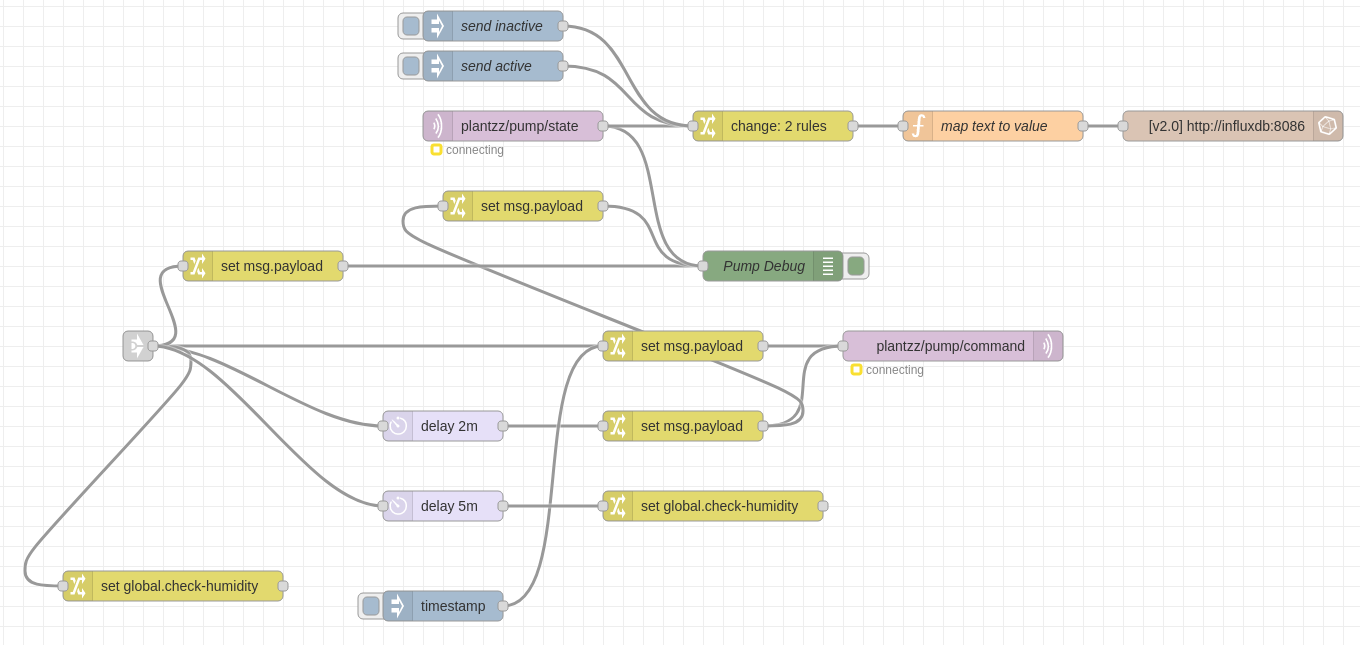
\includegraphics[width=\textwidth]{pump-control.png}
  \caption{Steuerungslogik für die Wasserpumpe in Node-RED}\label{fig:pump-control}
\end{figure}

Beim Starten der Steuerungslogik wird unmittelbar eine Nachricht mit dem Aktivierungskommando in dem MQTT-Topic der Pumpensteuerung veröffentlicht.
Zudem wird das globale Flag gesetzt, welches die die Überprüfungslogik deaktiviert.
Nach einer Verzögerung von zwei Minuten wird das Deaktivierungskommando veröffentlicht und nach fünf Minuten wird das Flag zur Deaktivierung der Überprüfungslogik wieder zurückgesetzt.

\subsection{Steuerung der Markise}

Neben der Wasserregelung soll das System fähig sein selbstständig zu überprüfen, ob eine Beschattung durch eine Markise momentan benötigt wird. Um  das Ein- und Ausfahren dieser Markise automatisch zu steuern, werden einige Umwelteinflüsse überprüft. Die Markise ist im Allgemeinen von der Sonneneinstrahlung abhängig. Weitere Faktoren, die ebenfalls zur Steuerung der Markise mit einbezogen werden, sind außerdem die Windgeschwindigkeit, die aus Wetterdaten entnommen wird, und die Umgebungstemperatur. 
Die folgende Abb. \ref{fig:canvas-activation} zeigt den entsprechenden Ablauf in Node-RED.

\begin{figure}[h]
  \centering
  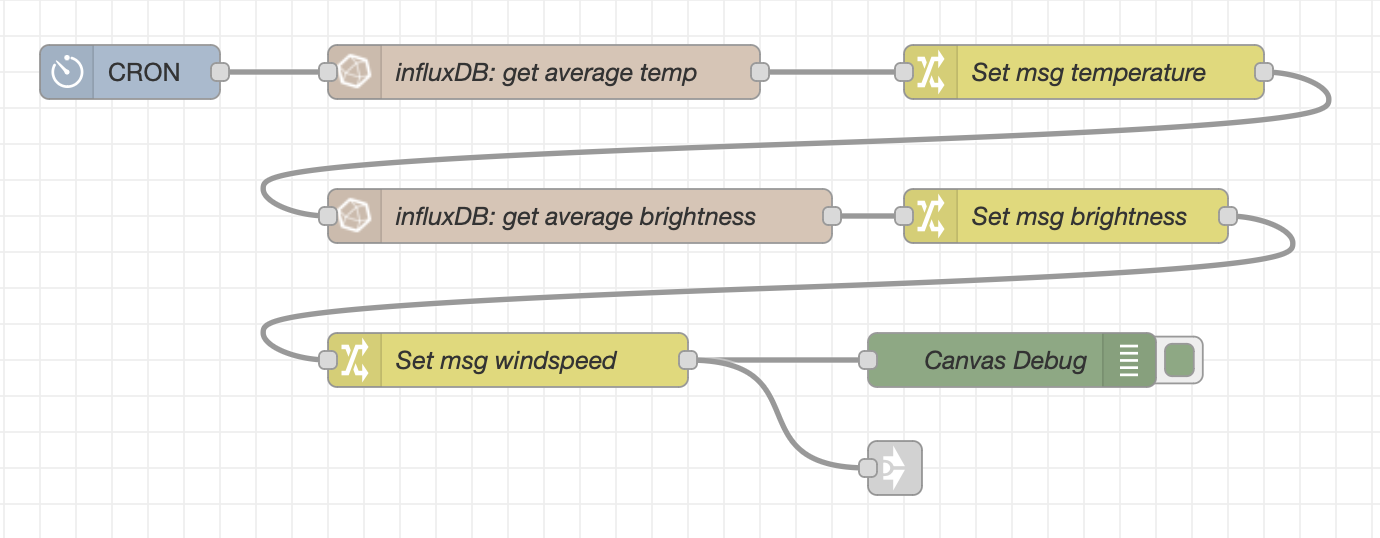
\includegraphics[width=\textwidth]{canvas-activation.png}
  \caption{Überprüfungslogik für die Markise in Node-RED}\label{fig:canvas-activation}
\end{figure}

Der Workflow startet, wie auch bei der Pumpensteuerung, mittels eines CRON-Triggers einmal pro Minute. Damit die Markise ausfährt werden hintereinander die Werte für die drei Kriterien ermittelt. 

Wenn der Durschnitt der Umgebungstemperatur in den letzten fünf Minuten über 20° Celsius liegt, ist der erste Check bestanden. Diese Grenze wurde eingeführt, da eine Beschattung im Sommer beziehungsweise bei hohen Temperaturen hilft, damit die Pflanzen nicht austrocken. Bei kälteren Temperaturen würde eine Beschattung wertvolle Sonnenstrahlen von den Pflanzen abhalten. Die zweite Überprüfung betrifft die Helligkeit, für welche ebenfalls der Durschnittswert der letzen fünf Minuten ausschlaggebend ist. Wenn dieser Wert über 15000 Lux liegt ist ein weiterer Kontrollpunkt überschritten. Der letzte Punkt, der noch überprüft wird, dient der Unversehrtheit der Markise. Die Markise darf nur ausfahren wenn die Windgeschwindigkeit von 14 m/s nicht überschritten ist.

Sind die drei Werte zur Überprüfung der Bedingungen ermittelt worden, so wird der Sub-Workflow zur Markisensteuerung angestoßen. Abb. \ref{fig:canvas-control} zeigt einen Ausschnitt aus Node-RED bezüglich des Sub-Workflows.

\begin{figure}[h]
  \centering
  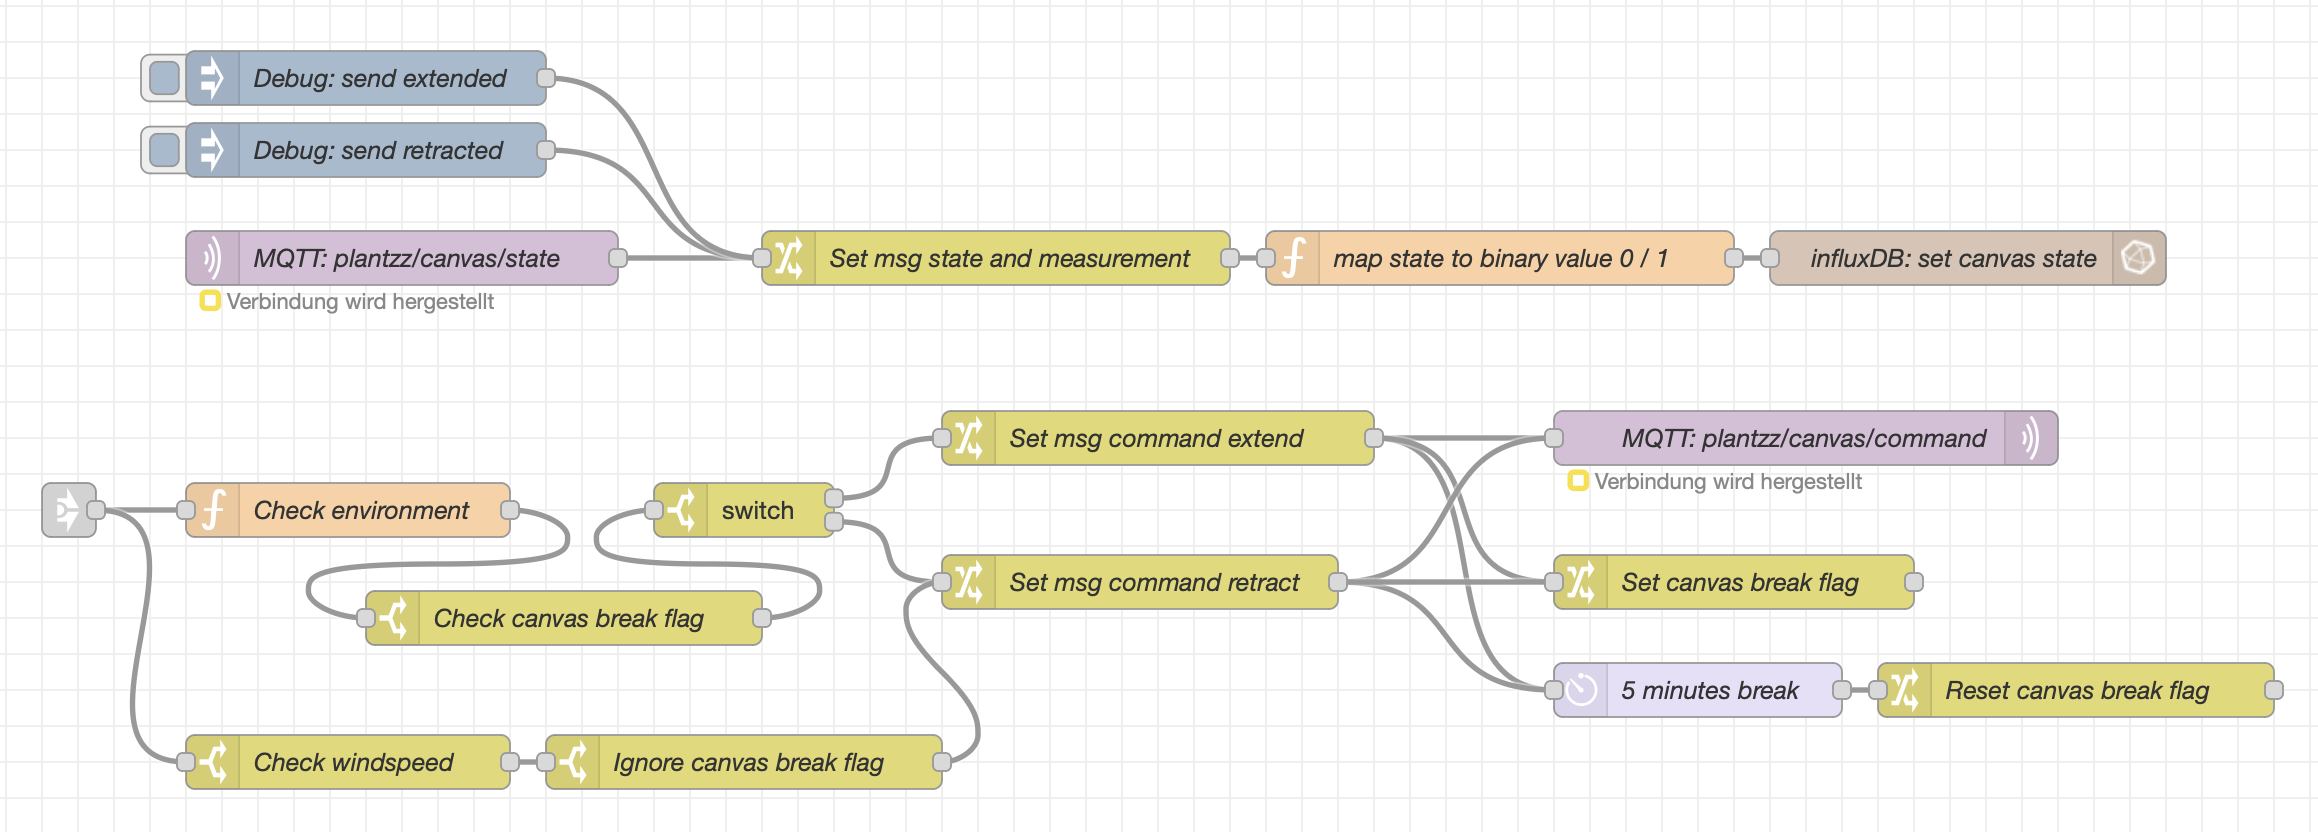
\includegraphics[width=\textwidth]{canvas-control.png}
  \caption{Steuerungslogik für die Markise in Node-RED}\label{fig:canvas-control}
\end{figure}

In der Funktion \texttt{Check environment} werden zunächst die bereits beschriebenen Checks durchgeführt. Danach wird abhängig vom Ergebnis der drei Überprüfungen entweder die Markise ein- oder ausgefahren.
Sobald der Befehl zum Ein- oder Ausfahren der Markise erteilt wurde, wird gleichzeitig die Freigabe zum erneuten Überprüfen der Markisensteuerung für fünf Minuten deaktiviert, um ein andauerndes Ein- und Ausfahren bei sich leicht ändernden Bedingungen im Grenzbereich zu verhindern. Parallel dazu wird die Windgeschwindigkeit als einzelnes Kriterium gesetzt, um die Markise bei Überschreiten des Grenzwerts sofort einfahren zu lassen, auch wenn das Flag zur Pause gesetzt ist.

\subsection{Einbindung eines Telegram Chat-Bots}

Zur Interaktion mit dem Nutzer wurde in der Applikationsschicht außerdem ein Telegram Chat-Bot implementiert. Über den Chat-Bot sind verschiedene Funktionen umsetzbar. Im Rahmen dieser Laborarbeit wurde ein Frostschutz umgesetzt: Sinkt die Bodentemperatur unter den Grenzwert von 3° Celsius, so erhält der Nutzer über den Messenger Telegram eine Warnung, dass der Boden droht zu gefrieren. Der Nutzer kann dadurch weitere Maßnahmen zum Schutz der Pflanzen einleiten. Die Definition dieser Funktion findet ebenfalls auf der Plattform Node-RED statt (siehe dazu Abb. \ref{fig:telegram}). In dem Funktionsblock \texttt{Build Telegram message} wird eine nutzerfreundliche Nachricht formuliert, welche als Push-Notification auf dem Smartphone des Nutzers erscheint.

\begin{figure}[h]
  \centering
  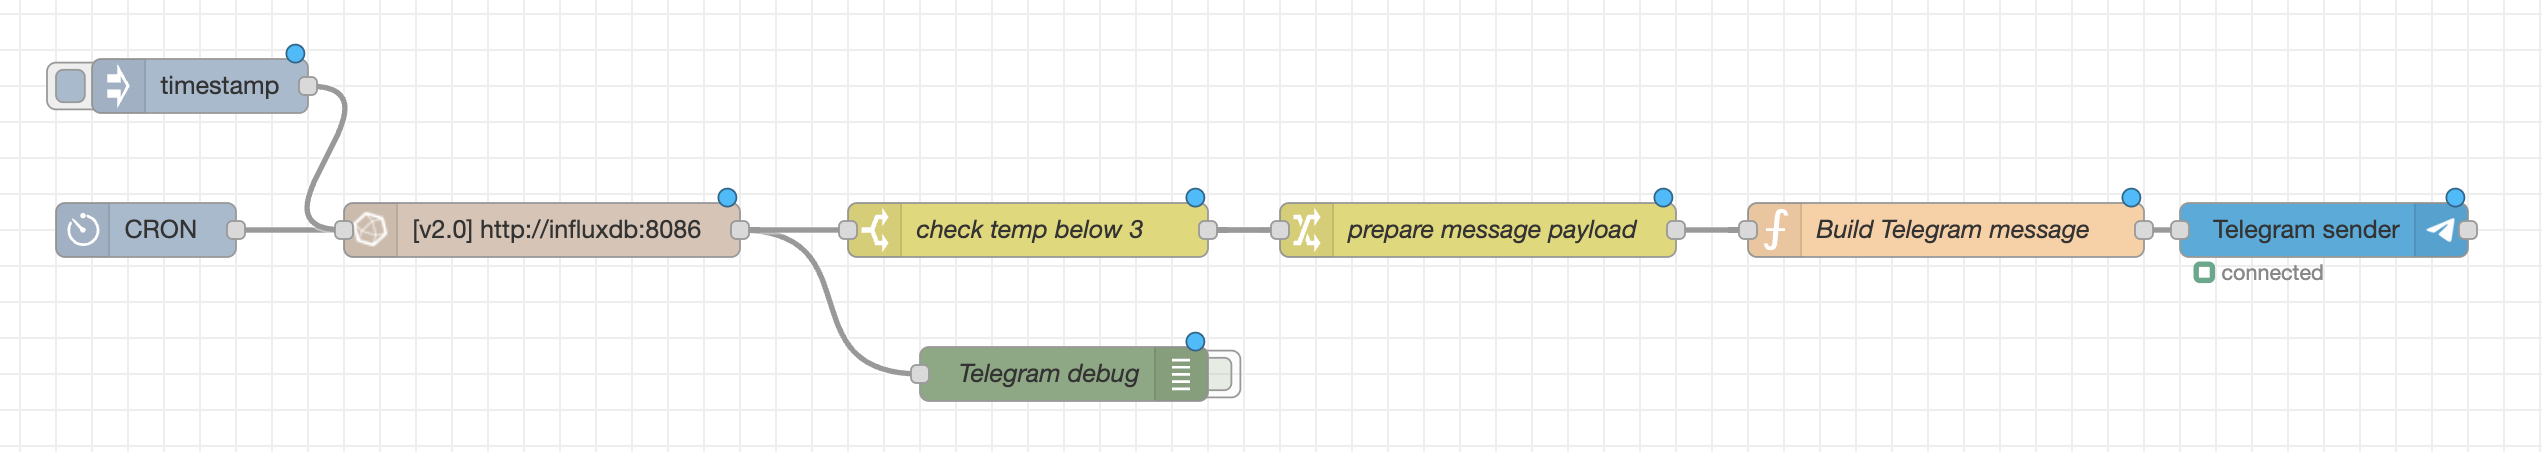
\includegraphics[width=\textwidth]{telegram.png}
  \caption{Einbindung von Telegram in Node-RED}\label{fig:telegram}
\end{figure}

Neben der Frostschutzfunktion können weitere Chat-Funktionen in Node-RED ausgestaltet werden. Zum Beispiel könnte der Nutzer über das Senden von gewissen Schlüsselwörtern das Ein- und Ausfahren der Markise manuell anstoßen. Die Umsetzung weiterer Chat-Funktionen wurde allerdings in der Laborarbeit nicht näher behandelt.

\subsection{Visualisierung in einem Grafana-Dashboard}

Der Nutzer soll einen Überblick erhalten, welche Temperatur und Luftfeuchtigkeit in seinem Garten vorliegt. Ebenso soll der aktuelle Zustand als auch der zeitliche Verlauf der Pumpe und der Markise einsehbar sein.
Für die Visualisierung der Sensorwerte als auch der Zustände der Aktoren wurde ein Grafana-Dashboard gebaut (siehe Abb. \ref{fig:grafana}). Durch das Deployment in einer Cloud-Infrastruktur lassen sich ortsunabhängig diese Werte einsehen, also bspw. auch wenn der Nutzer im Urlaub ist.

\begin{figure}[h]
  \centering
  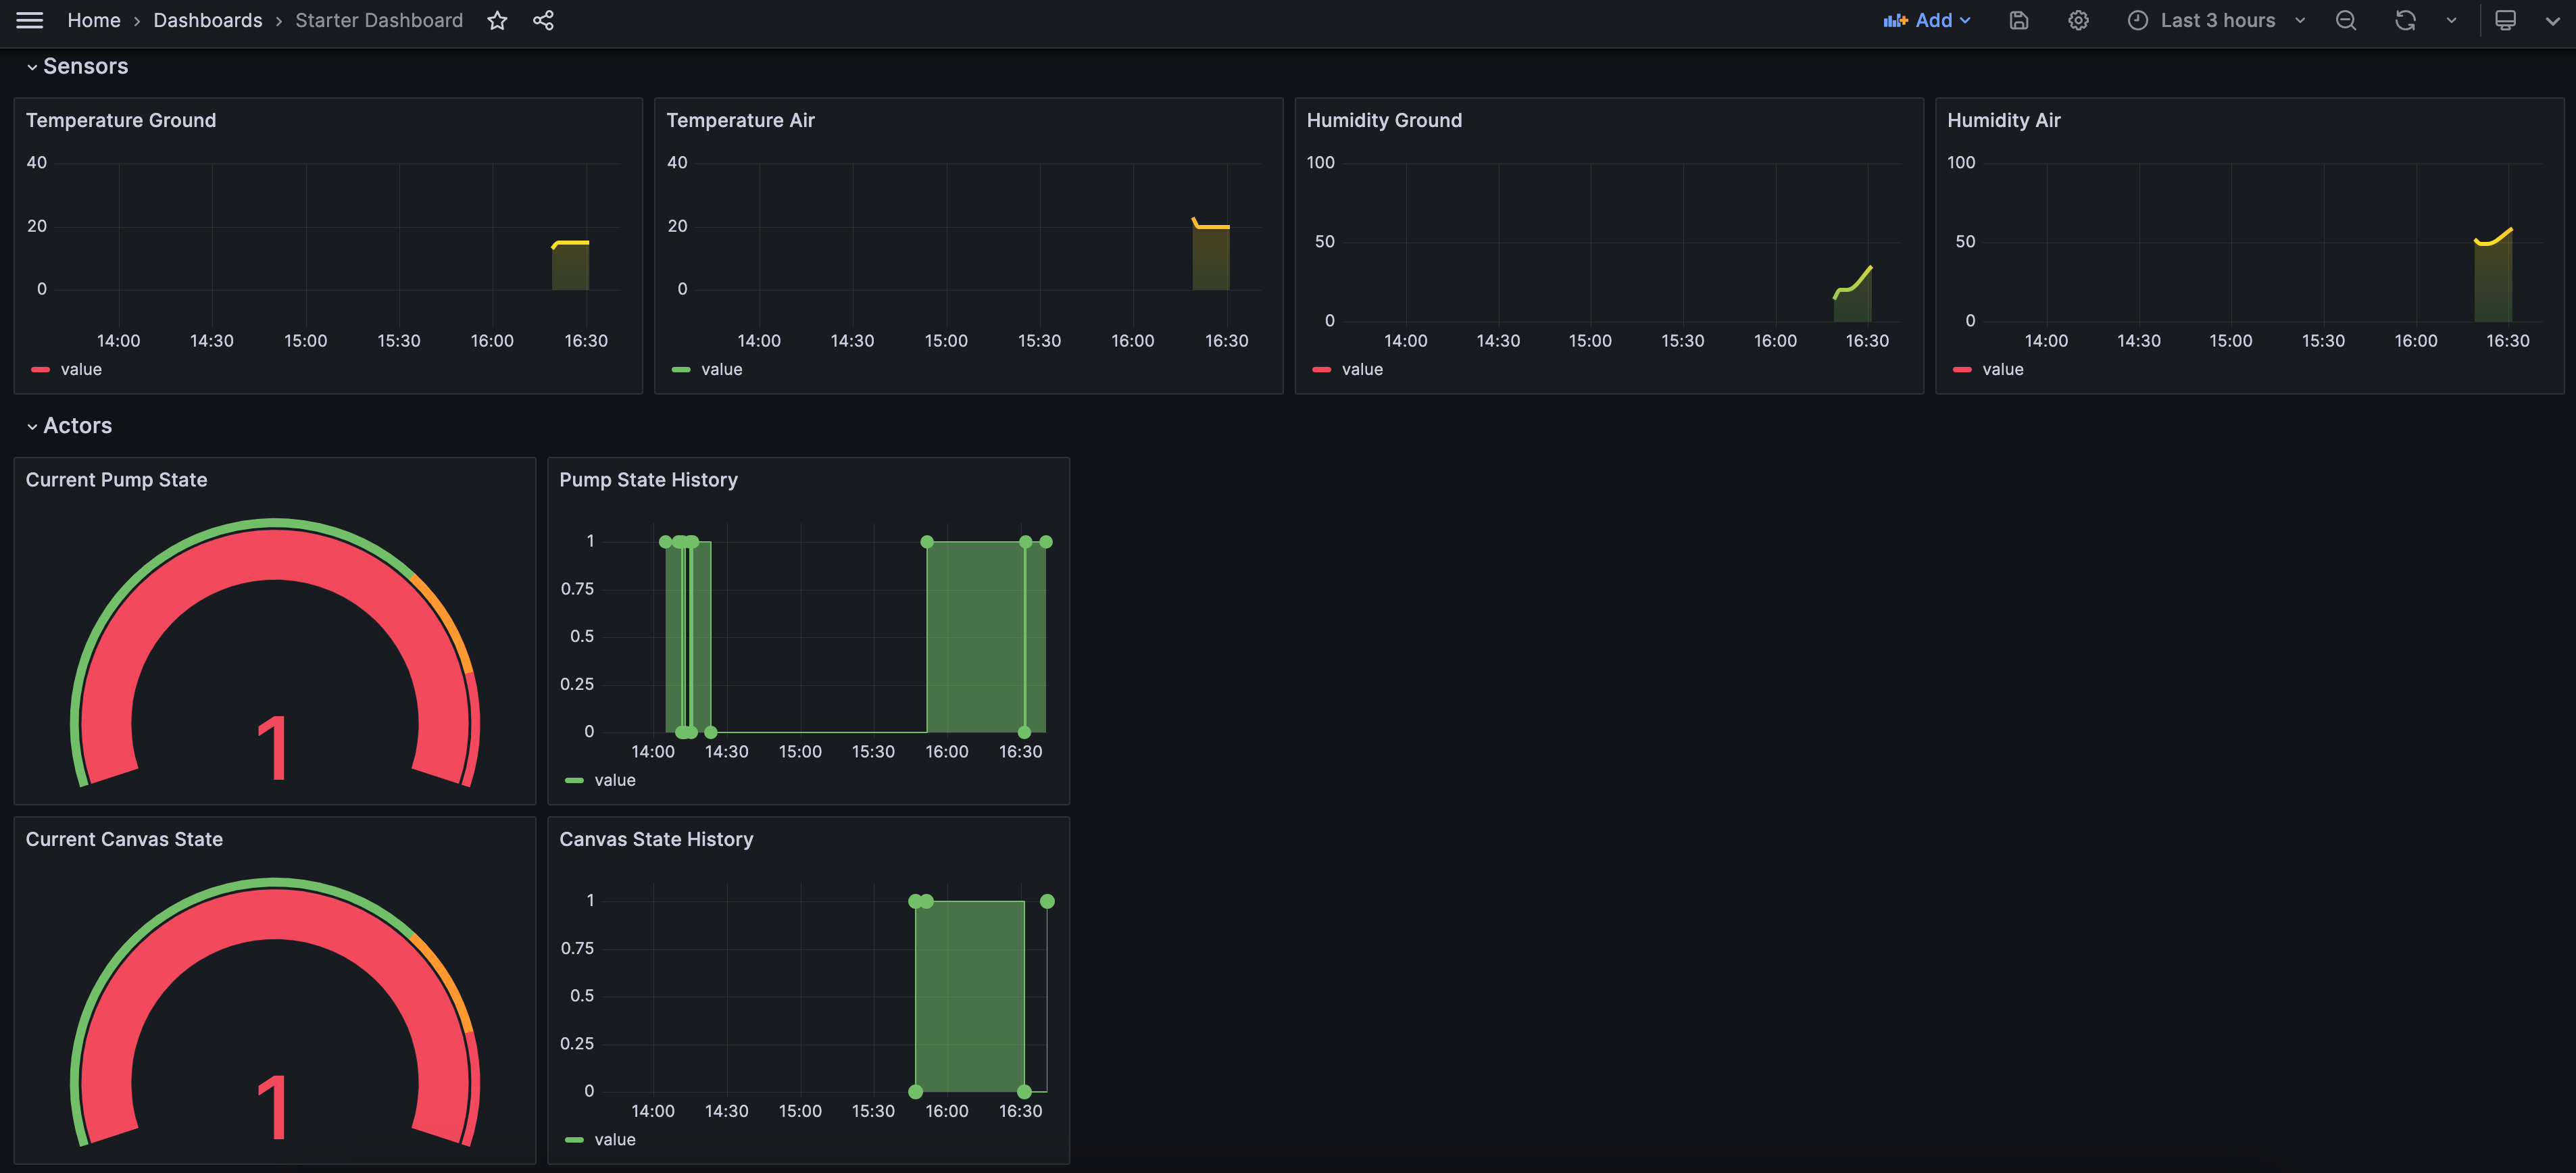
\includegraphics[width=\textwidth]{grafana.png}
  \caption{Dashboard in Grafana}\label{fig:grafana}
\end{figure}

Um die abgebildeten Daten in den verschiedenen Dashboard-Kacheln anzuzeigen, wurden mithilfe der Abfragesprache \textit{Flux} die relevanten Daten aus der Datenbank ausgelesen. 
Für den Aufbau des Dashboards wurde eine Connection zu der InfluxDB hergestellt. Per Default ist zum Zeitpunkt des Laborprojekts in Grafana die Version 1 von InfluxDB mit abweichend zu konfigurierenden Parametern hinterlegt. Da in diesem Laborprojekt die neuere Version 2 der InfluxDB eingesetzt wird, gilt es diese Version beim Aufbauen der Verbindung in Grafana zu berücksichtigen. 




% !TeX root = ../index.tex

\section{Fazit}
qqq

% BACKMATTER

\clearpage

% use roman numerals to number backmatter pages
\pagenumbering{Roman}

% use plain headers for backmatter pages
\pagestyle{plain.scrheadings}

% start numbering backmatter pages from 1
\setcounter{page}{\value{frontpagecount}}

% \pagestyle{empty}

% {
%   \centering\Huge\mbox{}
%   \vfill{}
%   Appendix\\
%   \vfill{}
% }

% \clearpage

\pagestyle{plain.scrheadings}

\appendix

% insert appendix sections here

\clearpage

% print bibliography in sloppypar environment for better URL placement
\begin{sloppypar}
  \printbibliography[
    heading=bibintoc % include bibliography in table of contents
  ]{}
\end{sloppypar}

\clearpage

\end{document}